\documentclass{standalone}
\usepackage{tikz}
\usetikzlibrary{patterns, positioning}
\usetikzlibrary{shapes.misc}
\usepackage[outline]{contour}
\contourlength{1.5pt} 


\begin{document}
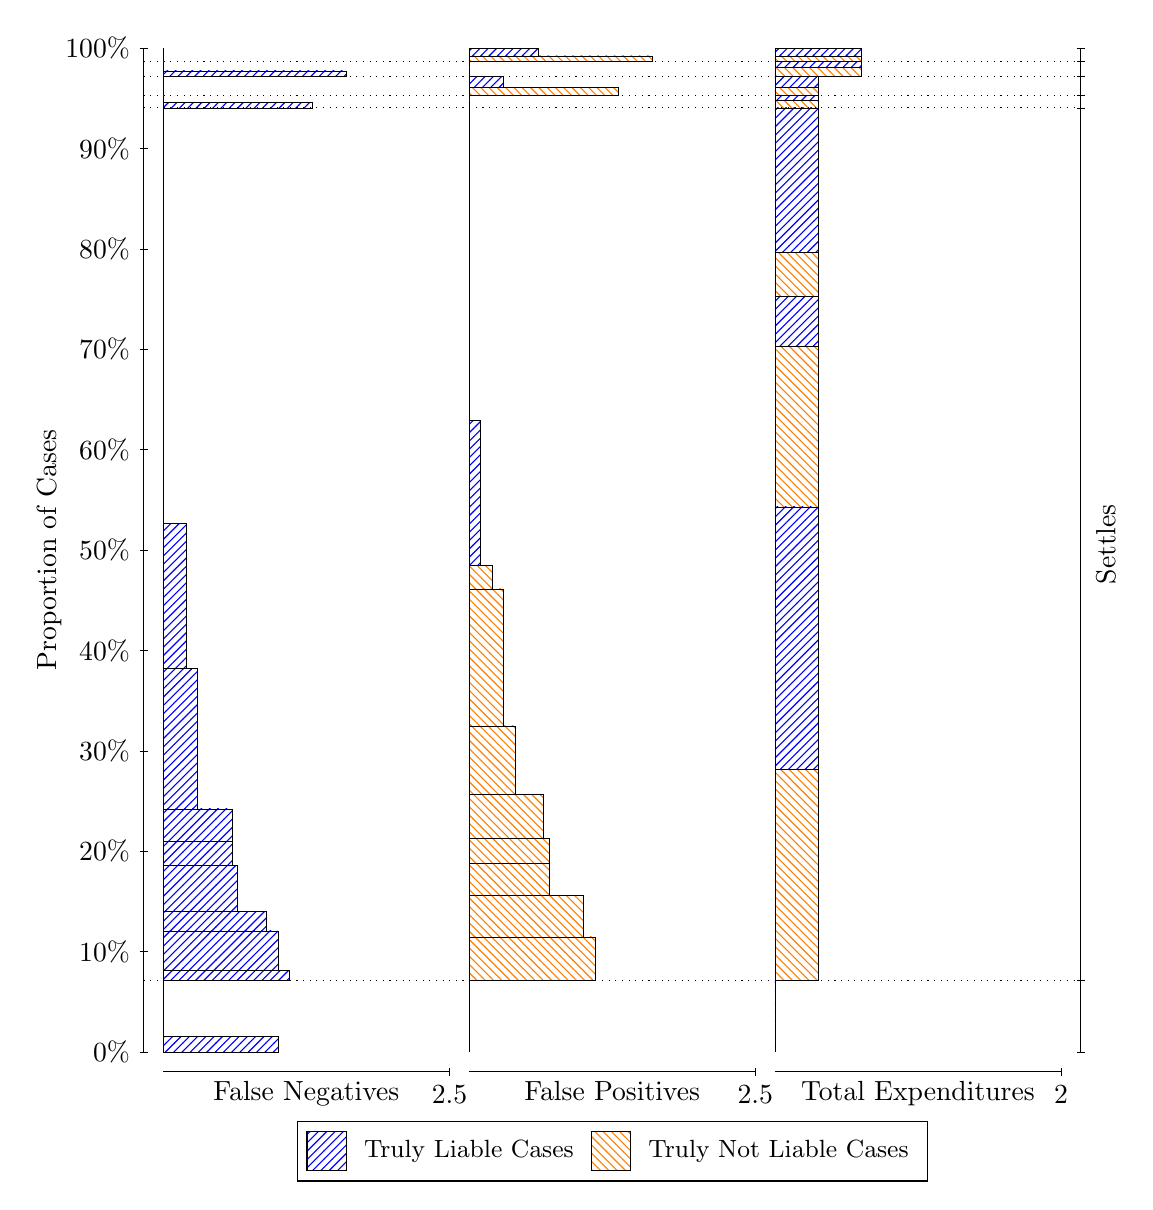
\begin{tikzpicture}
\draw[black, very thin] (1.5,1.75) -- (1.5,14.5);
\node[rotate=90, text=black, anchor=center] at (0.3, 8.125) {Proportion of Cases};
\draw[black, very thin] (1.45,1.75) -- (1.55,1.75);
\node[text=black, anchor=east] at (1.45, 1.75) {0\%};
\draw[black, very thin] (1.45,3.025) -- (1.55,3.025);
\node[text=black, anchor=east] at (1.45, 3.025) {10\%};
\draw[black, very thin] (1.45,4.3) -- (1.55,4.3);
\node[text=black, anchor=east] at (1.45, 4.3) {20\%};
\draw[black, very thin] (1.45,5.575) -- (1.55,5.575);
\node[text=black, anchor=east] at (1.45, 5.575) {30\%};
\draw[black, very thin] (1.45,6.85) -- (1.55,6.85);
\node[text=black, anchor=east] at (1.45, 6.85) {40\%};
\draw[black, very thin] (1.45,8.125) -- (1.55,8.125);
\node[text=black, anchor=east] at (1.45, 8.125) {50\%};
\draw[black, very thin] (1.45,9.4) -- (1.55,9.4);
\node[text=black, anchor=east] at (1.45, 9.4) {60\%};
\draw[black, very thin] (1.45,10.675) -- (1.55,10.675);
\node[text=black, anchor=east] at (1.45, 10.675) {70\%};
\draw[black, very thin] (1.45,11.95) -- (1.55,11.95);
\node[text=black, anchor=east] at (1.45, 11.95) {80\%};
\draw[black, very thin] (1.45,13.225) -- (1.55,13.225);
\node[text=black, anchor=east] at (1.45, 13.225) {90\%};
\draw[black, very thin] (1.45,14.5) -- (1.55,14.5);
\node[text=black, anchor=east] at (1.45, 14.5) {100\%};

\draw[black, very thin] (13.4,1.75) -- (13.4,14.5);
\draw[black, very thin] (13.35,1.75) -- (13.45,1.75);
\node[anchor=west] at (13.35, 1.75) {};
\draw[black, very thin] (13.35,2.6562) -- (13.45,2.6562);
\node[anchor=west] at (13.35, 2.6562) {};
\draw[black, very thin] (13.35,13.74) -- (13.45,13.74);
\node[anchor=west] at (13.35, 13.74) {};
\draw[black, very thin] (13.35,13.898) -- (13.45,13.898);
\node[anchor=west] at (13.35, 13.898) {};
\draw[black, very thin] (13.35,14.136) -- (13.45,14.136);
\node[anchor=west] at (13.35, 14.136) {};
\draw[black, very thin] (13.35,14.328) -- (13.45,14.328);
\node[anchor=west] at (13.35, 14.328) {};
\draw[black, very thin] (13.35,14.5) -- (13.45,14.5);
\node[anchor=west] at (13.35, 14.5) {};

\draw[black, very thin, pattern color=blue, pattern=north east lines] (1.75,1.75) rectangle (3.2033,1.9443);
\draw[black, very thin, pattern color=orange, pattern=north west lines] (1.75,1.9443) rectangle (1.75,2.6562);
\draw[black, very thin, pattern color=blue, pattern=north east lines] (1.75,2.6562) rectangle (3.3487,2.7911);
\draw[black, very thin, pattern color=blue, pattern=north east lines] (1.75,2.7911) rectangle (3.2033,3.2886);
\draw[black, very thin, pattern color=blue, pattern=north east lines] (1.75,3.2886) rectangle (3.058,3.5382);
\draw[black, very thin, pattern color=blue, pattern=north east lines] (1.75,3.5382) rectangle (2.6947,4.1199);
\draw[black, very thin, pattern color=blue, pattern=north east lines] (1.75,4.1199) rectangle (2.622,4.4289);
\draw[black, very thin, pattern color=blue, pattern=north east lines] (1.75,4.4289) rectangle (2.622,4.8373);
\draw[black, very thin, pattern color=blue, pattern=north east lines] (1.75,4.8373) rectangle (2.186,6.625);
\draw[black, very thin, pattern color=blue, pattern=north east lines] (1.75,6.625) rectangle (2.0407,8.4638);
\draw[black, very thin, pattern color=orange, pattern=north west lines] (1.75,8.4638) rectangle (1.75,13.74);
\draw[black, very thin, pattern color=blue, pattern=north east lines] (1.75,13.74) rectangle (3.6393,13.805);
\draw[black, very thin, pattern color=orange, pattern=north west lines] (1.75,13.805) rectangle (1.75,13.898);
\draw[black, very thin, pattern color=orange, pattern=north west lines] (1.75,13.898) rectangle (1.75,14.003);
\draw[black, very thin, pattern color=blue, pattern=north east lines] (1.75,14.003) rectangle (1.75,14.136);
\draw[black, very thin, pattern color=blue, pattern=north east lines] (1.75,14.136) rectangle (4.0753,14.211);
\draw[black, very thin, pattern color=orange, pattern=north west lines] (1.75,14.211) rectangle (1.75,14.328);
\draw[black, very thin, pattern color=orange, pattern=north west lines] (1.75,14.328) rectangle (1.75,14.4);
\draw[black, very thin, pattern color=blue, pattern=north east lines] (1.75,14.4) rectangle (1.75,14.5);
\draw[black, very thin, pattern color=orange, pattern=north west lines] (5.6333,1.75) rectangle (5.6333,2.4619);
\draw[black, very thin, pattern color=blue, pattern=north east lines] (5.6333,2.4619) rectangle (5.6333,2.6562);
\draw[black, very thin, pattern color=orange, pattern=north west lines] (5.6333,2.6562) rectangle (7.232,3.2102);
\draw[black, very thin, pattern color=orange, pattern=north west lines] (5.6333,3.2102) rectangle (7.0867,3.7377);
\draw[black, very thin, pattern color=orange, pattern=north west lines] (5.6333,3.7377) rectangle (6.6507,4.146);
\draw[black, very thin, pattern color=orange, pattern=north west lines] (5.6333,4.146) rectangle (6.6507,4.4621);
\draw[black, very thin, pattern color=orange, pattern=north west lines] (5.6333,4.4621) rectangle (6.578,5.0197);
\draw[black, very thin, pattern color=orange, pattern=north west lines] (5.6333,5.0197) rectangle (6.2147,5.8902);
\draw[black, very thin, pattern color=orange, pattern=north west lines] (5.6333,5.8902) rectangle (6.0693,7.6317);
\draw[black, very thin, pattern color=orange, pattern=north west lines] (5.6333,7.6317) rectangle (5.924,7.9329);
\draw[black, very thin, pattern color=blue, pattern=north east lines] (5.6333,7.9329) rectangle (5.7787,9.7717);
\draw[black, very thin, pattern color=blue, pattern=north east lines] (5.6333,9.7717) rectangle (5.6333,13.74);
\draw[black, very thin, pattern color=orange, pattern=north west lines] (5.6333,13.74) rectangle (5.6333,13.833);
\draw[black, very thin, pattern color=blue, pattern=north east lines] (5.6333,13.833) rectangle (5.6333,13.898);
\draw[black, very thin, pattern color=orange, pattern=north west lines] (5.6333,13.898) rectangle (7.5227,14.003);
\draw[black, very thin, pattern color=blue, pattern=north east lines] (5.6333,14.003) rectangle (6.0693,14.136);
\draw[black, very thin, pattern color=orange, pattern=north west lines] (5.6333,14.136) rectangle (5.6333,14.253);
\draw[black, very thin, pattern color=blue, pattern=north east lines] (5.6333,14.253) rectangle (5.6333,14.328);
\draw[black, very thin, pattern color=orange, pattern=north west lines] (5.6333,14.328) rectangle (7.9587,14.4);
\draw[black, very thin, pattern color=blue, pattern=north east lines] (5.6333,14.4) rectangle (6.5053,14.5);
\draw[black, very thin, pattern color=orange, pattern=north west lines] (9.5167,1.75) rectangle (9.5167,2.4619);
\draw[black, very thin, pattern color=blue, pattern=north east lines] (9.5167,2.4619) rectangle (9.5167,2.6562);
\draw[black, very thin, pattern color=orange, pattern=north west lines] (9.5167,2.6562) rectangle (10.062,5.3363);
\draw[black, very thin, pattern color=blue, pattern=north east lines] (9.5167,5.3363) rectangle (10.062,8.6726);
\draw[black, very thin, pattern color=orange, pattern=north west lines] (9.5167,8.6726) rectangle (10.062,10.715);
\draw[black, very thin, pattern color=blue, pattern=north east lines] (9.5167,10.715) rectangle (10.062,11.348);
\draw[black, very thin, pattern color=orange, pattern=north west lines] (9.5167,11.348) rectangle (10.062,11.902);
\draw[black, very thin, pattern color=blue, pattern=north east lines] (9.5167,11.902) rectangle (10.062,13.74);
\draw[black, very thin, pattern color=orange, pattern=north west lines] (9.5167,13.74) rectangle (10.062,13.833);
\draw[black, very thin, pattern color=blue, pattern=north east lines] (9.5167,13.833) rectangle (10.062,13.898);
\draw[black, very thin, pattern color=orange, pattern=north west lines] (9.5167,13.898) rectangle (10.062,14.003);
\draw[black, very thin, pattern color=blue, pattern=north east lines] (9.5167,14.003) rectangle (10.062,14.136);
\draw[black, very thin, pattern color=orange, pattern=north west lines] (9.5167,14.136) rectangle (10.607,14.253);
\draw[black, very thin, pattern color=blue, pattern=north east lines] (9.5167,14.253) rectangle (10.607,14.328);
\draw[black, very thin, pattern color=orange, pattern=north west lines] (9.5167,14.328) rectangle (10.607,14.4);
\draw[black, very thin, pattern color=blue, pattern=north east lines] (9.5167,14.4) rectangle (10.607,14.5);
\draw[black, dotted] (1.5,2.6562) -- (13.4,2.6562);
\draw[black, dotted] (1.5,13.74) -- (13.4,13.74);
\draw[black, dotted] (1.5,13.898) -- (13.4,13.898);
\draw[black, dotted] (1.5,14.136) -- (13.4,14.136);
\draw[black, dotted] (1.5,14.328) -- (13.4,14.328);
\draw[black, very thin] (1.75,1.5) -- (5.3833,1.5);
\node[text=black, anchor=north] at (3.5667, 1.5) {False Negatives};
\draw[black, very thin] (5.3833,1.45) -- (5.3833,1.55);
\node[text=black, anchor=north] at (5.3833, 1.45) {2.5};

\draw[black, very thin] (5.6333,1.5) -- (9.2667,1.5);
\node[text=black, anchor=north] at (7.45, 1.5) {False Positives};
\draw[black, very thin] (9.2667,1.45) -- (9.2667,1.55);
\node[text=black, anchor=north] at (9.2667, 1.45) {2.5};

\draw[black, very thin] (9.5167,1.5) -- (13.15,1.5);
\node[text=black, anchor=north] at (11.333, 1.5) {Total Expenditures};
\draw[black, very thin] (13.15,1.45) -- (13.15,1.55);
\node[text=black, anchor=north] at (13.15, 1.45) {2};


\node[text=black, centered, rotate=90] at (13.72, 8.1983) {\contour{white}{Settles}};





\draw (7.449999999999999,1.5) node[draw=none] (baseCoordinate) {};
\begin{scope}[align=center]
        \matrix[scale=0.5, draw=black, below=0.5cm of baseCoordinate, nodes={draw}, column sep=0.1cm]{
            \node[rectangle, draw, minimum width=0.5cm, minimum height=0.5cm, pattern color=blue, pattern=north east lines] {}; &
            \node[draw=none, font=\small, text=black] (B) {Truly Liable Cases}; &
            \node[rectangle, draw, minimum width=0.5cm, minimum height=0.5cm, pattern color=orange, pattern=north west lines] {}; &
            \node[draw=none, font=\small, text=black] (B) {Truly Not Liable Cases}; \\
            };
\end{scope}

\end{tikzpicture}
\end{document}